\chapter{Additional Clustering and Visualization}\label{chapter:grovercode}

The original vision of OverCode was to discover pedagogically valuable themes of variation within thousands of student solutions to the same programming exercise. While OverCode does normalize and cluster correct solutions so that they can be more easily understood as a group, it does not pull out larger themes of variation as clearly as initially hoped for, nor does it handle incorrect solutions. This chapter describes more recent efforts to address both these shortcomings.

\section{Clustering Solutions with Statistical Models}\label{sec:latent}

One approach to pulling out larger themes of variation within solutions is to cluster more aggressively. OverCode's existing clustering pipeline is a form of deterministic interpretable clustering. What can vary and what is invariant across all the solutions within a cluster is clear, just by reading the normalized solution that represents the cluster. Because it faithfully represents the syntax students used in each cluster, solutions are split apart into smaller clusters by small syntactic differences. 

One promising set of methods for more aggressive groupings of solutions are bottom-up and built on rules. Specifically, these methods define rules for which solutions or groups of solutions can be merged into a single cluster. Probablistic semantic equality or equality with respect to a teacher's test suite, which is already used by OverCode for variable names, can be used for subexpressions as well~\cite{}. Methods built on program language analysis and synthesis, such as compiler optimizations, could collapse OverCode clusters based on known semantic equality. As a system designer, one must decide or give the teacher control over how many different, semantically equivalent solutions are collapsed into a single cluster since, at the highest level, all correct solutions to the same programming exercise are semantically equivalent. These methods are discussed again in the future work, because the second set of methods were chosen for future investigation in this chapter.

The second set of methods leverage statistical properties of the entire corpus of solutions. Given that Variation Theory is interested in dimensions of variation (and consistency) that characterize all possible instantiations of an idea, statistical methods warrant further investigation. Latent variable models are a type of statistical model that attempt to explain variation in a dataset based on underlying factors. With the right choice of features and model, a latent variable model may be able to capture underlying design choices. In this section, two latent variable models have been explored in a preliminary way for this purpose: the Bayesian Case Model (BCM)~\cite{} and Latent Dirichlet Allocation (LDA)~\cite. 

BCM was selected because, like the original OverCode pipeline, it clusters solutions and produces a single solution to represent the entire cluster. Like OverCode, it also indicates the features that characterize each cluster. While OverCode displays the set of normalized lines that all members of a cluster deterministically share, BCM learns a subspace of features that are most characteristic of the solutions within cluster, in a probabilistic sense. It also has an interactive variant called iBCM, which allows the user to directly modify the prototype and the subspace chosen by BCM if it disagrees with their domain knowledge or preferences. This user modification triggers a rerun of BCM with the modifications taken into account.%is taken into account by the algorithm 

Internally, BCM depends on a mixture model with a Dirichlet prior. Rather than find a cluster for each entire solution, mixture models can learn clusters of features that co-exist across some subset of all solutions. The concentration parameter of BCM's Dirichlet prior is set to promote sparsity, i.e., mixture distributions over solutions that have the majority of their probability mass on a single mixture component. BCM then assigns each solution to a cluster according to its most probable mixture component. %In other words, after fitting the model to the data, each solution will likely have a single dominant mixture component associated with it. If data points were documents instead of solutions, one would say that each document is determined to have a single dominating topic.

LDA was selected as an alternative statistical approach to BCM because of evidence collected at UCBerkeley~\cite{} that experts were themselves not particularly consistent about how to cluster solutions. While LDA's output is not as optimized for interpretability as BCM's, it preserves the ability to examine solutions through the lens of their mixture components, rather than clusters. LDA learns both mixture components, which are distribution over features, and the distributions of those mixtures over each solution in the set it is trained on. Depending on the features chosen to represent solutions, it may be difficult to interpret exactly what a mixture component is just by looking at its distribution over features. However, sorting solutions based on the degree to which a particular topic is associated with them may pull out a distinctive, human-interpretable themes. %Furthermore, when using LDA, the concentration parameter of the Dirichlet prior need not promote for sparsity; it can be tuned by a human or a heuristic, to maximize the usefulness of the resulting breakdown into mixture components. This parameter's optimal value may be problem-specific and teacher-specific. 



\subsection{Interpretable Clustering Solutions with BCM}

BCM was applied to the normalized cluster-representing solutions generated by OverCode. These normalized solutions encode both static and dynamic information in a readable function, i.e., the syntax carries the static information and the variable name encodes dynamic information. The normalized function body is tokenized and represented as binary vectors indicating  the existence of the features, including renamed variables and language-specific keywords, such as specific normalized variable names like \texttt{listA} and Python keywords like \texttt{assert} and \texttt{while}. The result is a BCM clustering of OverCode clusters.

In a small pilot study, three introductory Python teachers were each given sets of Python solutions to three different programming problems selected from those previously analyzed in the chapter on OverCode. For each problem, they were asked to create a grading rubric and provide helpful comments for the students, based on interacting with solutions in one of three different interfaces. The three interfaces were: (1) raw solutions in the browser, similar to the control used in the OverCode studies, (2) OverCode's normalized cluster-representating solutions, and (3) a BCM clustering of OverCode clusters, i.e., the prototypes and characteristic features of each BCM cluster, as well as its cluster members. The BCM interface, shown in Figure~\ref{overcode_ibcm}, was running the iBCM variant of the algorithm, so teachers could promote a member of a cluster to be its prototype or click on a token within a prototype--a variable name or keyword--to toggle whether or not it is considered a characteristic feature of that cluster. Both these modifications triggered BCM running in the backend to rerun and send a new clustering to the front end for display. 

Pilot users appreciated the fact that BCM gave some structure to the space of solutions. Rather than a long list of solutions, the interface suggested distinct subpopulations of solutions within the list. However, subjects did not fully understand the probabilistic nature of the clustering method. The presence of a single intruder, i.e., a solution that the teacher believed did not belong in a cluster, caused confusion. This could be ameliorated by giving users more ways to modify the clustering, e.g., allowing users the option to kick an intruder out of a cluster and rerun BCM, or by introducing the tool as a mechanism for discovery instead of organization. Subjects also requested richer or higher-level features than variable names and keywords. Kim's PhD thesis~\cite{beenthesis} describes a follow-up full user study comparing the efficacy of BCM vs. iBCM on clustering OverCode cluster-representing solutions.

\begin{figure}[ht]
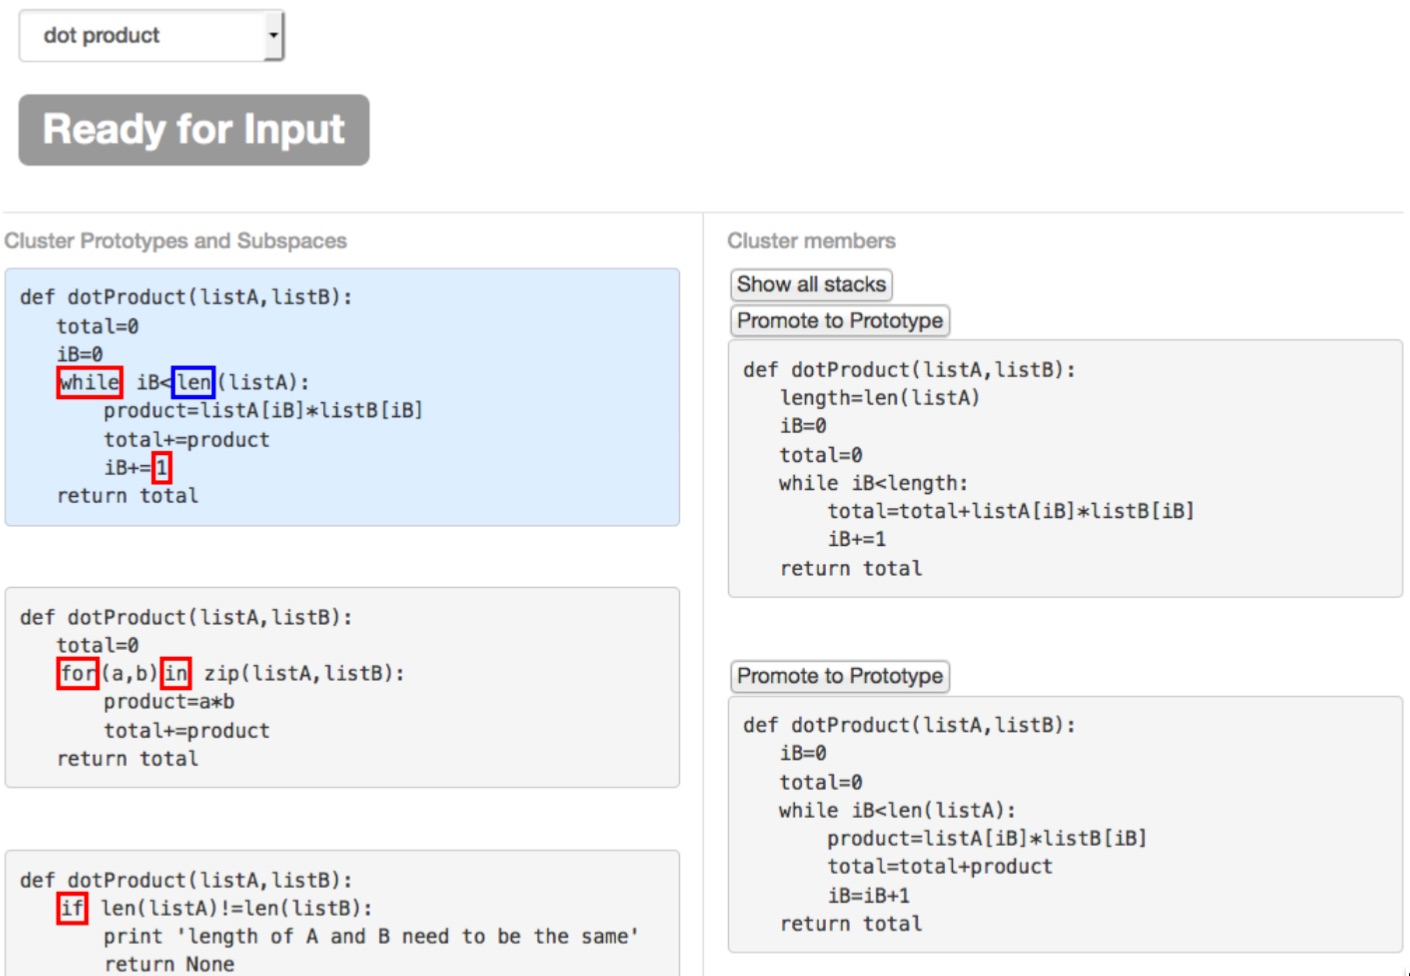
\includegraphics[width=0.75\columnwidth]{Body/figures/grovercode/overcode_ibcm}
\caption{The solutions on the left are cluster prototypes. The blue solution is the selected cluster whose members are shown in a scrollable list on the right hand side. The tokens contained in red boxes are features that BCM identifies as characteristic of the cluster represented by that prototype. When a user hovers their cursor over a keyword or variable name, e.g., \texttt{len}, it is highlighted in a blue rectangle, indicating that it can be interacted with, i.e., clicked.}
\label{overcode_ibcm}
\end{figure} 

\subsection{Mixture Modeling Solutions with LDA}

As described in the chapter on related work, other researchers have documented a lack of agreement across human-made clusters of student code. One possible explanation for this low consistency across teacher-made clusterings of student code is that solutions are mixtures of design choices and teachers care about different things. As described in~\cite{berkeleymastersthesis}: the clusters can be as straight forward as "1 pt", "2 pts" and "3 pts". If student A writes a solution with a well-written loop and extraneous statements while student B writes a solution with extra loops but otherwise very clean code, teachers can reasonably disagree about which cluster each whole solution should be placed in, depending on whether they believe inefficient control flow or extraneous statements are worse.

Instead of trying to approximate clusterings that humans do not even agree on, it may be more useful to model solutions as mixtures of good and bad design choices. While more sophisticated mixture models' assumptions may ultimately be more appropriate, LDA \cite{lda} as implemented in the Gensim toolbox \cite{gensim} was chosen as the model to evaluate in this preliminary work. 

Like BCM, LDA was run on the normalized cluster-representing solutions, not raw solutions. However, the representation of these solutions was also changed: in order to pull out higher-level patterns in approach, rather than lower-level patterns in syntax, solutions were represented solely by the behavior of the variables within them. 

As described in the chapter on OverCode, the OverCode analysis pipeline executes all programs on a common set of test cases and records the sequence of values taken on by each variable in the program. OverCode assumes that variables in different programs that transition through the same sequence of values on the same test cases are in fact fulfilling the same semantic role in the program. %This sequence of values taken on by each variable in each program becomes a signature, i.e., the key to recognizing semantically equivalent variables across programs.  % and can therefore be considered the same {\bf common variable} uniquely defined by that sequence of values.



\begin{figure}[ht]
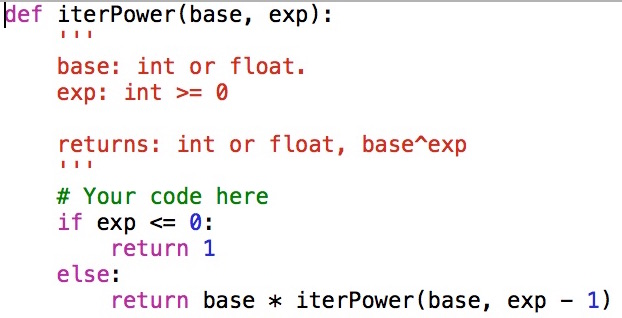
\includegraphics[width=0.75\columnwidth]{Body/figures/grovercode/recursive_example}
\caption{Example of a recursive student solution.}
\label{recursive_example}
\vspace*{\floatsep}
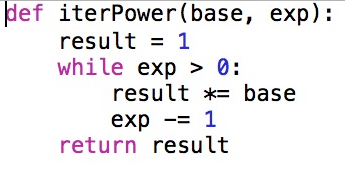
\includegraphics[width=0.45\columnwidth]{Body/figures/grovercode/whilestandard}
\caption{Example of a student solution using the Python keyword \texttt{while}.}
\label{whilestandard}
\vspace*{\floatsep}
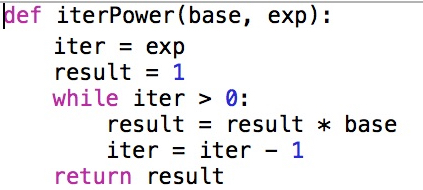
\includegraphics[width=0.5\columnwidth]{Body/figures/grovercode/augmentedwhile}
\caption{Example of a student solution using the Python keyword \texttt{while}, where the student has not modified any input arguments, i.e., better programming style.}
\label{augmentedwhile}
\end{figure} 

Below are the sequences of variable values recorded by OverCode while executing \texttt{iterPower(5,3)} as defined in Figures \ref{recursive_example}, \ref{whilestandard}, and \ref{augmentedwhile}:
\begin{itemize}
  \item {\bf Figure \ref{recursive_example}}
  \begin{itemize}
  \setlength\itemsep{0.05em}
  \item \texttt{exp: 3, 2, 1, 0, 1, 2, 3}
  \item \texttt{base: 5}
  \end{itemize}
  \item {\bf Figure \ref{whilestandard}}
  \begin{itemize}
  \item \texttt{exp: 3, 2, 1, 0}
  \item \texttt{base: 5}
  \item \texttt{result: 1, 5, 25, 125}
  \end{itemize}
  \item {\bf Figure \ref{augmentedwhile}}
  \begin{itemize}
  \item \texttt{exp: 3}
  \item \texttt{base: 5}
  \item \texttt{iter: 3, 2, 1, 0}
  \item \texttt{result: 1, 5, 25, 125}
  \end{itemize}
\end{itemize}

In the previous examples, the input argument \texttt{base} would be considered variable common to all three programs, but the input argument \texttt{exp} would not be. The variable \texttt{result} would also be considered a common variable shared across just the definitions in Figure \ref{whilestandard} and Figure \ref{augmentedwhile}. This allows us to distinguish between programs that calculate the answer in semantically distinct ways, without discriminating between the low-level design decisions about syntax. 

LDA is often applied to corpora of textual documents, where the corpus is represented as a $W \times N$ term-by-document matrix of counts, where $W$ is the vocabulary size across all documents and $N$ is the number of documents. In this representation, the document is represented a bag of word counts, i.e., how many times each word appears in the document. Following this analogy, solutions are represented as a bag of variable behaviors. The matrix representing the solutions in Figures \ref{recursive_example} through \ref{augmentedwhile} executed on \texttt{iterPower(5,3)} is shown in Table \ref{varbydocmat}.

\begin{table}[t]
\caption{Variable-by-Solution Matrix for Programs, where variables are uniquely identified by their sequence of values while run on a set of test case(s)}
\label{varbydocmat}
%\vskip 0.15in
\begin{center}
\begin{small}
\begin{sc}
\begin{tabular}{| l | c | c | c | c | c |}
\hline
%\abovespace\belowspace
Sol- & \texttt{5} & \texttt{1,5,...} & \texttt{3,2,1,0,} & \texttt{3,2,1,0} & \texttt{3} \\
ution& & \texttt{25,125} & \texttt{...1,2,3} & &  \\
\hline
%\abovespace
Fig. \ref{recursive_example} & 1 & 0 & 1 & 0 & 0 \\
Fig. \ref{whilestandard}     & 1 & 1 & 0 & 1 & 0 \\
Fig. \ref{augmentedwhile}    & 1 & 1 & 0 & 1 & 1 \\
\hline
\end{tabular}
\end{sc}
\end{small}
\end{center}
%\vskip -0.1in
\end{table}

Note that, while the entries in Table \ref{varbydocmat} only take on values $0$ or $1$, more complicated definitions may have $n$ instances of, e.g., a variable that takes on the sequence of values \texttt{3,2,1,0}. In that case, there could be an $n$ in the \texttt{3,2,1,0} column for the row corresponding to that solution, or it can be left as a binary indicator. %In other words, true to the assumptions made by LDA, these are occurrence counts, not binary indicators.

%\subsection{Procedure}

In order to run LDA, 3875 student solutions to \texttt{iterPower} were first run on a set of test cases within the OverCode analysis pipeline. The OverCode pipeline produced a set of 977 cluster-representing solutions and a set of features for each solution, including which variable sequences were observed during execution. Another script turned this output into a variable-by-solution matrix for the 977 cluster-representing solutions, which were then fed into LDA for analysis. LDA was run repeatedly with multiple values for the parameter that sets the number of latent mixture components. The results were examined by hand since perplexity and held-out likelihoods are not necessarily good proxies for human interpretability \cite{readingtealeaves}. 

Since the learned mixture components are distributions over variable behaviors, it is easier to inspect solutions which have high amounts of that mixture component within them and infer a theme by comparing them to solutions that contain high amounts of a different mixture component. These comparisons were done by hand for a subset of popular mixture components for each LDA model. One topic comparison captured the difference between solutions like Figure ~\ref{augmentedwhile} and ~\ref{whilestandard}. Another topic comparison exposed the difference between the subpopulation of solutions with extra (unnecessary) conditional statements and the common, more concise solution. In the future, a user interface would be very helpful for this task, especially one which made it easier to compare the output of models with different parameter values. 

LDA applied to a variable-by-solution matrix is a promising method for identifying variation within corpora of solutions to the same programming exercise. However, LDA's assumptions, such as the independence of mixture components, and requirements, such as explicitly setting the number of mixture components beforehand, may mean that other mixture models, such as the Correlated Topic Model~\cite{} or the Hierarchical Dirichlet Process~\cite{} will ultimately be a better model fit for this purpose.



\section{Conclusion}
The clustering described in the original OverCode work was relatively limited in scope, but it did produce, at least for simple introductory Python programming problems, a concise standardized representation of solutions that can be used for more statistically sophisticated clustering techniques and as a starting point for helping graders understand and grade incorrect student solutions by hand.

